\chapter{Background}

In this chapter a theoretical background of electrical conductivity measurement will be established. After that, a market research takes a look at the commercially available solutions of sensor systems and parts that could be used to develop one.

\section{Theoretical Background}

The following section is translated and summarized from \textcite{trankler2015sensortechnik} and \textcite{gevatter2000automatisierungstechnik}.\\

The conductivity $ \kappa $  is the ability of a certain volume of a substance to conduct electricity. It is measured in the unit \unitfrac{S}{m} and is a specific parameter normalized to the length and cross section of the volume. Conductivity in a liquid depends on ions as charge carrier and can therefore be used to measure its concentration.

To better understand conductivity, an equivalent circuit diagram, shown in figure \ref{fig:ecd}, of an electrode system shown in figure \ref{fig:elec}, can be used. This method is called conductometry and in this form a two-electrode-cell is used. In this measurement configuration, two electrodes are submerged in the liquid to be measured and a voltage is applied. The resistance $ R $ of the substance is determined by measuring the potential drop $U_R$ given a constant voltage $ U $, current $ I $ and internal resistance $ R_i$. \\

\begin{figure}
	\begin{center}
		\begin{circuitikz}[european voltages]
			\draw
  			(0,0) to [short, *-] (2,0)
  			to [R, l=$R$] (2,2)
  			(0,0) to [open, v^<=$U$] (0,4)
  			to [short, *- ,i=$I$] (2,4)
  			to [R, l_=$R_i$] (2,2)
  			(2.25,0) to [open, v<=$U_R$] (2.25,2);
		\end{circuitikz}
		\caption[The equivalent circuit diagram.]{The equivalent circuit diagram shows the voltage drop $U_R$ over the resistance of the fluid relative to the internal resistance $R_i$, driven by the applied voltage $U$.}
		\label{fig:ecd}
	\end{center}
\end{figure}

\begin{figure}
	\begin{center}
    	\tikzset{external/export next=false}
		\begin{tikzpicture}
  		    % Draw electrode
 	   		\fill [black!25] (0.5,2) node[left, black] {$A$} rectangle (1.5,-1);
	    		% draw voltmeter
 	   		\draw[join = round, thick] (1,2) -- (1,2.5) -- (2.4,2.5);
 	   		\draw[join = round, thick] (3.1,2.5) -- (4.5,2.5) -- (4.5,2);
 	   		\draw (2.75,2.5) node [circle, draw] {V};
  	  		%Draw electrode
  	  		\fill [black!25] (4,2) node[left, black] {$A$}  rectangle (5,-1);
  	  		
		\draw [darrow] (1.5,-0.5) -- (4,-0.5) node[above, pos=0.5] {$d$};
    		%Draw water
    		\fill [blue!75, opacity=0.3] (-0.5,1) rectangle (6,-2);
		\end{tikzpicture}
		\caption[Two electrodes submerged in the solution.]{Two electrodes with the area $A$ are submerged in the solution with the distance $d$ between them. A voltmeter is used to measure the voltage drop.}
		\label{fig:elec}
	\end{center}
\end{figure}

The resistance $ R $ is
\begin{equation}
	R = \dfrac{U_R}{I}
\label{eq:R}
\end{equation}

The inverse of the resistance $ R $ is the conductance $ G $
\begin{equation}
	G = \dfrac{I}{U_R}
\label{eq:G}
\end{equation}

The cell constant $ C $ describes the geometry of the sensor
\begin{equation}
	C = \dfrac{d}{A}
\label{eq:C}
\end{equation}
where $ d $ is the distance between and $ A $ the surface area of  the electrodes. 

Considering the cell constant $ C $ finally yields the conductivity
\begin{equation}
	\kappa = G \cdot C
\label{eq:kappa} 
\end{equation}
\\

In electrolytes, the electrical conduction is a result of mass transfer, where ions are carrying the charges. If the measurement is conducted with direct current, this mass transfer leads to changes in the measured solution and the electrode surface, negatively impacting the measurement. Furthermore, polarization effects create additional resistance, leading to lower than actual results. To avoid this, alternating current is used. The fast, periodical swap of polarity eliminates the net mass flow and its effects. Polarization is a result of the current flowing through the electrode, thereby its effects can be minimized by minimizing this current. One method to do this is replacing the two-electrode-cell with a four-electrode-cell.
This separates the current flow from the potential measurement by using one electrode pair to apply the current, and a separate pair to measure the potential drop. \\

The electrolyte's temperature affects the mobility of the ions and thereby also has a big influence on the conductivity. It has to be taken into account when comparing two measurements. If the temperature $ T $ is known, the conductivity at that temperature $ \kappa_{T} $ can be normalized to a reference temperature $ T_{ref} $ using equation \eqref{eq:kref}, resulting in the reference conductivity $ \kappa_{ref} $.

\begin{equation}
	\kappa_{ref} = \kappa_{T} \frac{1}{1 + C_{T} \cdot (T - T_{ref})}
\label{eq:kref}
\end{equation}

The temperature coefficient $ C_{T} $ assumes a linear correlation and is only valid in a narrow temperature range. For bigger ranges the denominator can be replaced with a polynomial using higher order coefficients, resulting in equation \eqref{eq:kref+}.

\begin{equation}
	\kappa_{ref} = \kappa_{T} \frac{1}{\sum\limits_{i=0}^n C_{Ti} \cdot (T - T_{ref})^{i}}
\label{eq:kref+}
\end{equation}

\section{Market Research}

Conductivity meters can be readily bought and range from prices of over \euro{1000} for lab equipment \parencite{expcm} to \euro{100} for simple field water quality monitors \parencite{cheapcm}. Even cheaper water quality testers from no-name manufacturers can be found for as little as \euro{10} from online vendors.

\begin{figure}[H]
	\begin{center}
    	\tikzset{external/export next=false}
		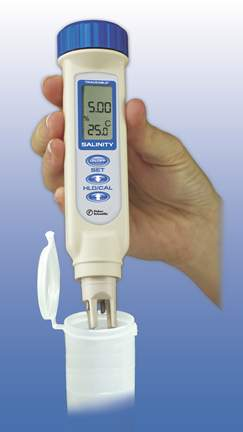
\includegraphics[scale=0.5]{images/ccm.jpg}
		\caption{Fisher Scientific™ Traceable™ Salinity Meter Pen \parencite{cheapcm}}
		\label{fig:ccm}
	\end{center}
\end{figure}

Figure \ref{fig:ccm} shows a field conductivity meter from a quality manufacturer as example for the typical traits most available solutions share:
\begin{itemize}
	\item a single electrode pair
	\item a display to report measurements
	\item designed to perform singular reads with high quality
\end{itemize}

While field conductivity meters have the electrodes integrated to form one compact device, the more expensive lab equipment often has the electrodes attached to the device with a cable, allowing for a more flexible use.\\

A different option was found in the MinieC I2C eC interface from Sparky's Widgets \parencite{uec}. The MinieC interface is an Open Hardware project providing a conductivity sensor that easily interfaces with a microcontroller, licensed under Creative Commons \parencite{cc}. This license allows to study the original design files and build modified versions. Ready-made boards can be purchased for about \euro{25}. The design approach of this solution is also more modular than that of the more professional equipment. The MinieC offers an interface to connect external electrodes and can be controlled and read by a microcontroller.\\

Table \ref{tab:feat} shows a comparison of the strengths and weaknesses of the different systems with respect to the use case in this project. Both the lab and field conductivity meters offer complete solutions with high accuracy. They do however lack the modularity of the MinieC as well as the machine interface, both of which are more important for the intended purpose than the accuracy. The complete solutions they offer simply are solutions for a different case than ours, while the MinieC is positioned as a flexible building block to be used in whatever way needed. While it means that more work has to be done in designing a system around it, this is exactly the trait that allows us to build a device fit for our tasks.

\begin{table}[H]
    \centering

    \caption[]{Feature comparison table of different conductivity sensor solutions. Strengths and weaknesses are indicated by + and - signs.}
    \label{tab:feat}
    \begin{tabular}{l  c  c  c}
        	\toprule
         Feature & Lab Conductivity Meter & Field Conductivity Meter & MinieC \\
        	\midrule
		Price & - - & - & + \\
		Modularity & - & - - & ++ \\
		Completeness & ++ & ++ & - \\
		Interface & - & - & ++ \\
		Accuracy & ++ & + & - \\
        \bottomrule
    \end{tabular}
\end{table}